\documentclass{article}
\usepackage{graphicx}
\usepackage{hyperref}
\usepackage{caption}
\usepackage{subcaption}
\usepackage{mathtools}
\usepackage[dutch]{babel}

\begin{document}

\begin{center}
	\huge{Wiskunde in Kunst}\\
	\LARGE{Opdracht 10} \\
	
	\vspace{2cm}
	
	\Large{Fractals en de Gulden Snede}\\
	
	\vfill
	
	\begin{figure}[Hh]
		\centering
		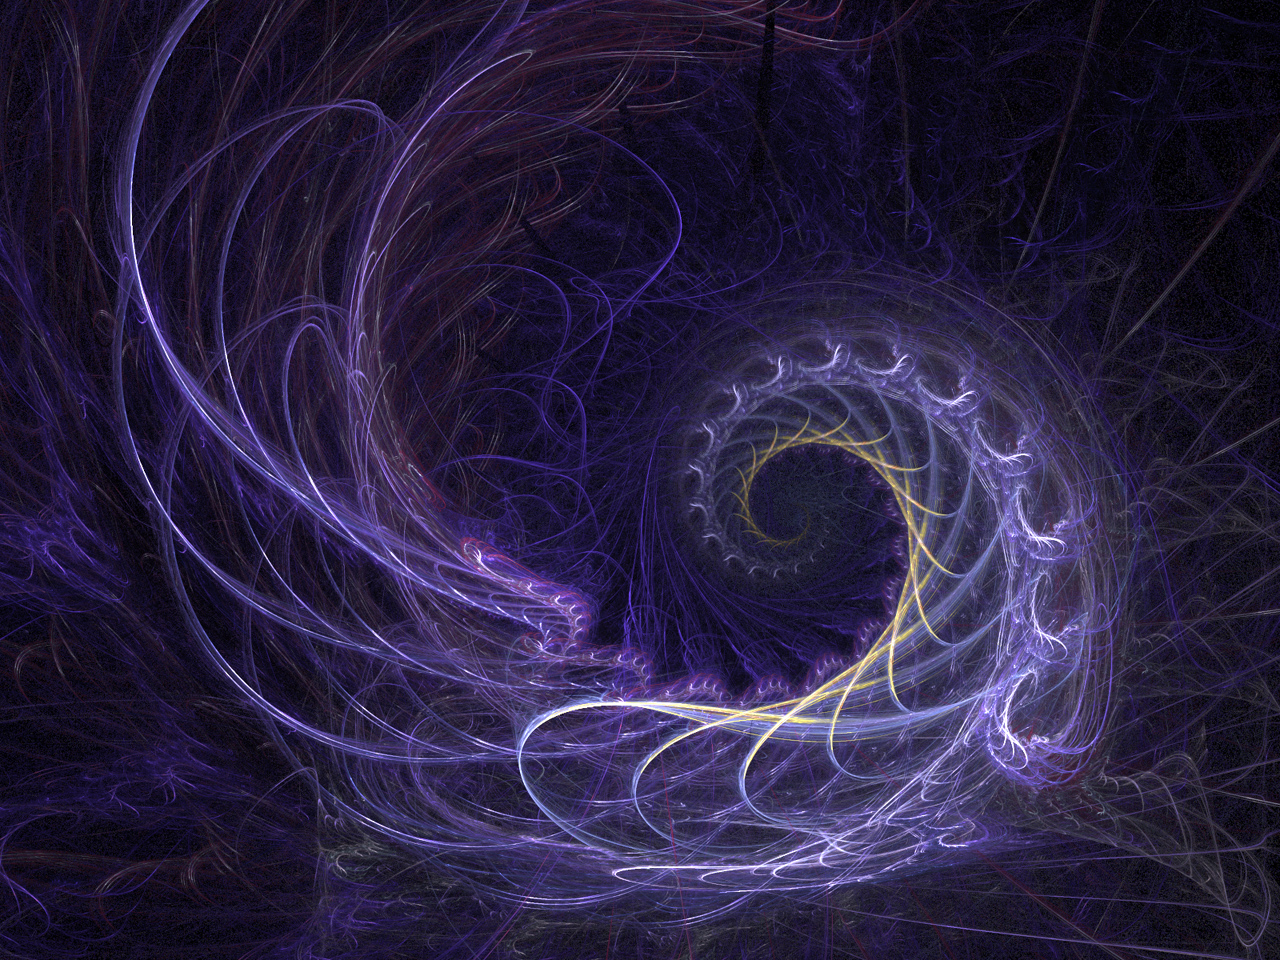
\includegraphics[width=\textwidth]{Golden_Ratio.jpg}
	\end{figure}
	
	\vfill
	\Large{Marcelo Dias Avelino} \hfill \large{0840416}
\end{center}

\thispagestyle{empty} % Remove page numbering

\pagebreak

\setcounter{page}{1} % Start counting pages here

\section{De relatie}

Zoals uitgelegd in de vorige verslagen, een fractal is een figuur die opgebouwd is uit delen dat min of meer gelijk zijn aan het algemene figuur. Fractals hebben oneindig veel detailles en kunnen oneindig worden ingezoomd zonder enige detail te verliezen. Ze zijn opgebouwd uit een set regels en waardes en \'e\'en van die waardes is de gulden snede.

% \begin{figure}[Hh]
% 	\centeringuit
% 	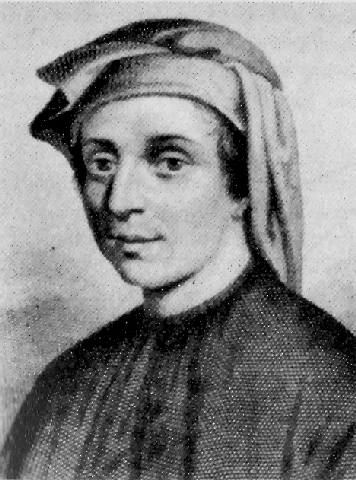
\includegraphics[width=0.3\textwidth]{Fibonacci.jpg}
% 	\caption{Portret van Fibonnaci door onbekende auteur.}
% \end{figure}

\end{document}
